% DynamicMCPBench --- EMNLP 2026 Industry Track poster.
% Gemini beamerposter theme (ITMO fork). Build with the Makefile (lualatex):
%   make            % -> poster.pdf
% Size: A0 portrait (841 x 1189 mm), the ACL/EMNLP de-facto poster standard.
% Visual-first layout: 2 wide columns, large figures, minimal text, one QR.

\documentclass[final]{beamer}

% ====================
% Packages
% ====================

\usepackage[T1]{fontenc}
\usepackage{lmodern}
\usepackage[size=a0,orientation=portrait,scale=1.25]{beamerposter}
\usetheme{gemini}
\usecolortheme{cam}
\usepackage{graphicx}
\usepackage{booktabs}
\usepackage{tikz}
\usepackage{qrcode}
\usepackage{anyfontsize}

% ====================
% Lengths --- 2 columns
% ====================

% (N+1)*sepwidth + N*colwidth = paperwidth
\newlength{\sepwidth}
\newlength{\colwidth}
\setlength{\sepwidth}{0.03\paperwidth}
\setlength{\colwidth}{0.455\paperwidth}

\newcommand{\separatorcolumn}{\begin{column}{\sepwidth}\end{column}}

% ====================
% Title
% ====================

\title{DynamicMCPBench: A Trace-Grounded, Effect-Scored Benchmark\\
  for LLM Agents over Live MCP Servers}

\author{%
  Jerzy Kami\'nski\textsuperscript{1},
  Ilya Galyukshev\textsuperscript{1,2},
  Artem Kuznetsov\textsuperscript{1},
  Sergey Chuprin\textsuperscript{1},
  Kirill Redko\textsuperscript{1},
  Aidar Shumbalov\textsuperscript{1},
  Anna Kalyuzhnaya\textsuperscript{1}}

\institute[ITMO]{%
  \textsuperscript{1}ITMO University \samelineand
  \textsuperscript{2}Central University}

\footercontent{
  \href{https://github.com/ITMO-NSS-team/DynamicMCPBench}{github.com/ITMO-NSS-team/DynamicMCPBench} \hfill
  EMNLP 2026 Industry Track --- Budapest \hfill
  \href{mailto:jkaminski@niuitmo.ru}{jkaminski@niuitmo.ru}}

\logoleft{
\includegraphics[height=5cm]{logos/itmo-logo-2.pdf}}
\logoright{
\includegraphics[height=4cm]{logos/ENG_CU_logo_white.png}}

\begin{document}

\begin{frame}[t]
\begin{columns}[t]
\separatorcolumn

% ==================== COLUMN 1 ====================
\begin{column}{\colwidth}

  \begin{block}{Grade effects, not answers}

    Answer-matching and fixed tool lists break on live, stateful MCP servers. We
    record successful agent traces, distill them into path-agnostic
    \textbf{effect checkpoints}, and grade an agent only on whether it
    \emph{reproduces those effects} --- never on the answer string.

  \end{block}

  \begin{block}{The pipeline}
    \begin{figure}
      \centering
      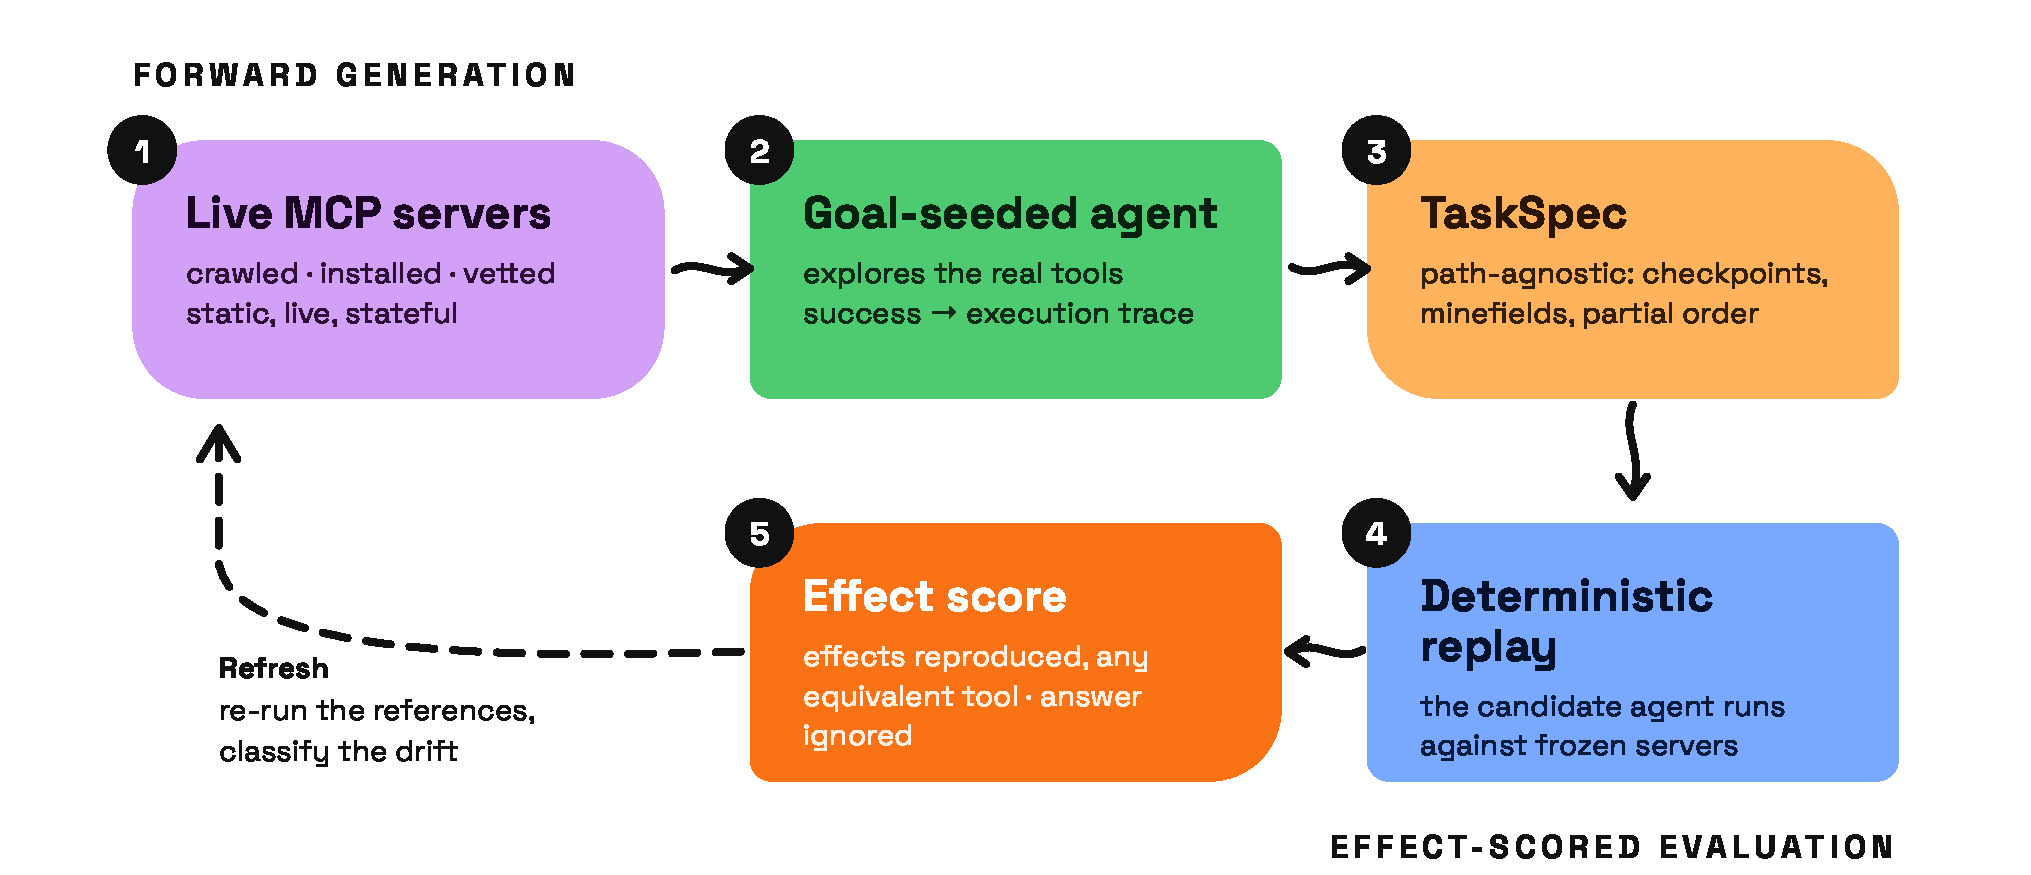
\includegraphics[width=\colwidth]{figures/fig_pipeline_v2.pdf}
    \end{figure}
    \vspace{-0.5em}
    {\small Five automated stages. \textbf{(1)}~Crawl and vet live MCP servers,
    tagging each tool as live-read or stateful-write. \textbf{(2)}~A goal-seeded
    agent explores the real tools and records a successful execution trace.
    \textbf{(3)}~The trace is distilled into a TaskSpec: path-agnostic effect
    checkpoints, equivalence sets, minefields, and a partial order.
    \textbf{(4)}~Candidates run under deterministic replay against frozen
    servers. \textbf{(5)}~Effects are scored --- any equivalent tool accepted,
    the answer ignored. A refresh loop re-runs the references to track drift.}
  \end{block}

  \begin{alertblock}{How scoring works}

    \begin{itemize}
      \item \textbf{Effect checkpoints} with \textbf{equivalence sets}: any tool
        that produces the required effect passes, so different valid routes all
        count.
      \item \textbf{Minefields}: forbidden actions fail the run.
      \item \textbf{Tier-1, deterministic} (no model, no network); scored
        \textbf{pass\textasciicircum{}3} --- solved only if 3/3 attempts pass.
    \end{itemize}

  \end{alertblock}

  \begin{block}{The benchmark}

    DynamicMCPBench measures whether a configured agent completes multi-step
    goals across live services. We score \textbf{24 models} on \textbf{750
    tasks} (15 categories $\times$ 50) over \textbf{121 live MCP servers}, drawn
    from a \textbf{1{,}168-tool} catalog. Every task is a real, replayable
    trajectory, and the framework regenerates on \emph{your own} servers.

  \end{block}

  \begin{block}{Capability is not bought by size}
    \begin{figure}
      \centering
      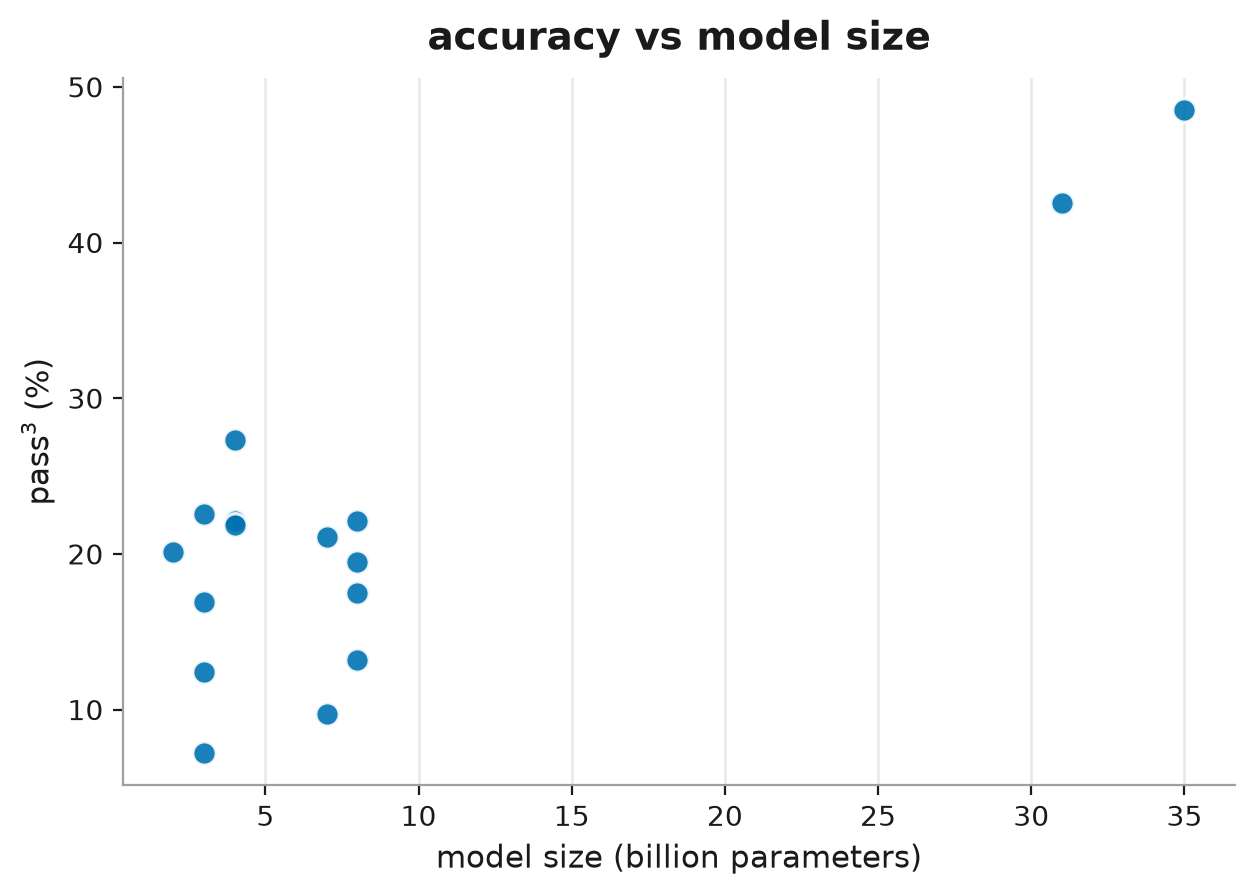
\includegraphics[width=0.58\colwidth]{figures/fig_size.png}
    \end{figure}
    \vspace{-0.4em}
    {\small Below ${\sim}30$B parameters a 4B model outperforms every 7--8B one:
    training and architecture matter more than raw scale.}
  \end{block}

  \begin{block}{Validated against humans}

    Annotators confirmed \textbf{94.9\%} of the scorer's passes; the error is
    one-sided, so read every score as a \textbf{lower bound} on true capability.

  \end{block}

\end{column}

\separatorcolumn

% ==================== COLUMN 2 ====================
\begin{column}{\colwidth}

  \begin{block}{The benchmark is far from solved}
    \begin{figure}
      \centering
      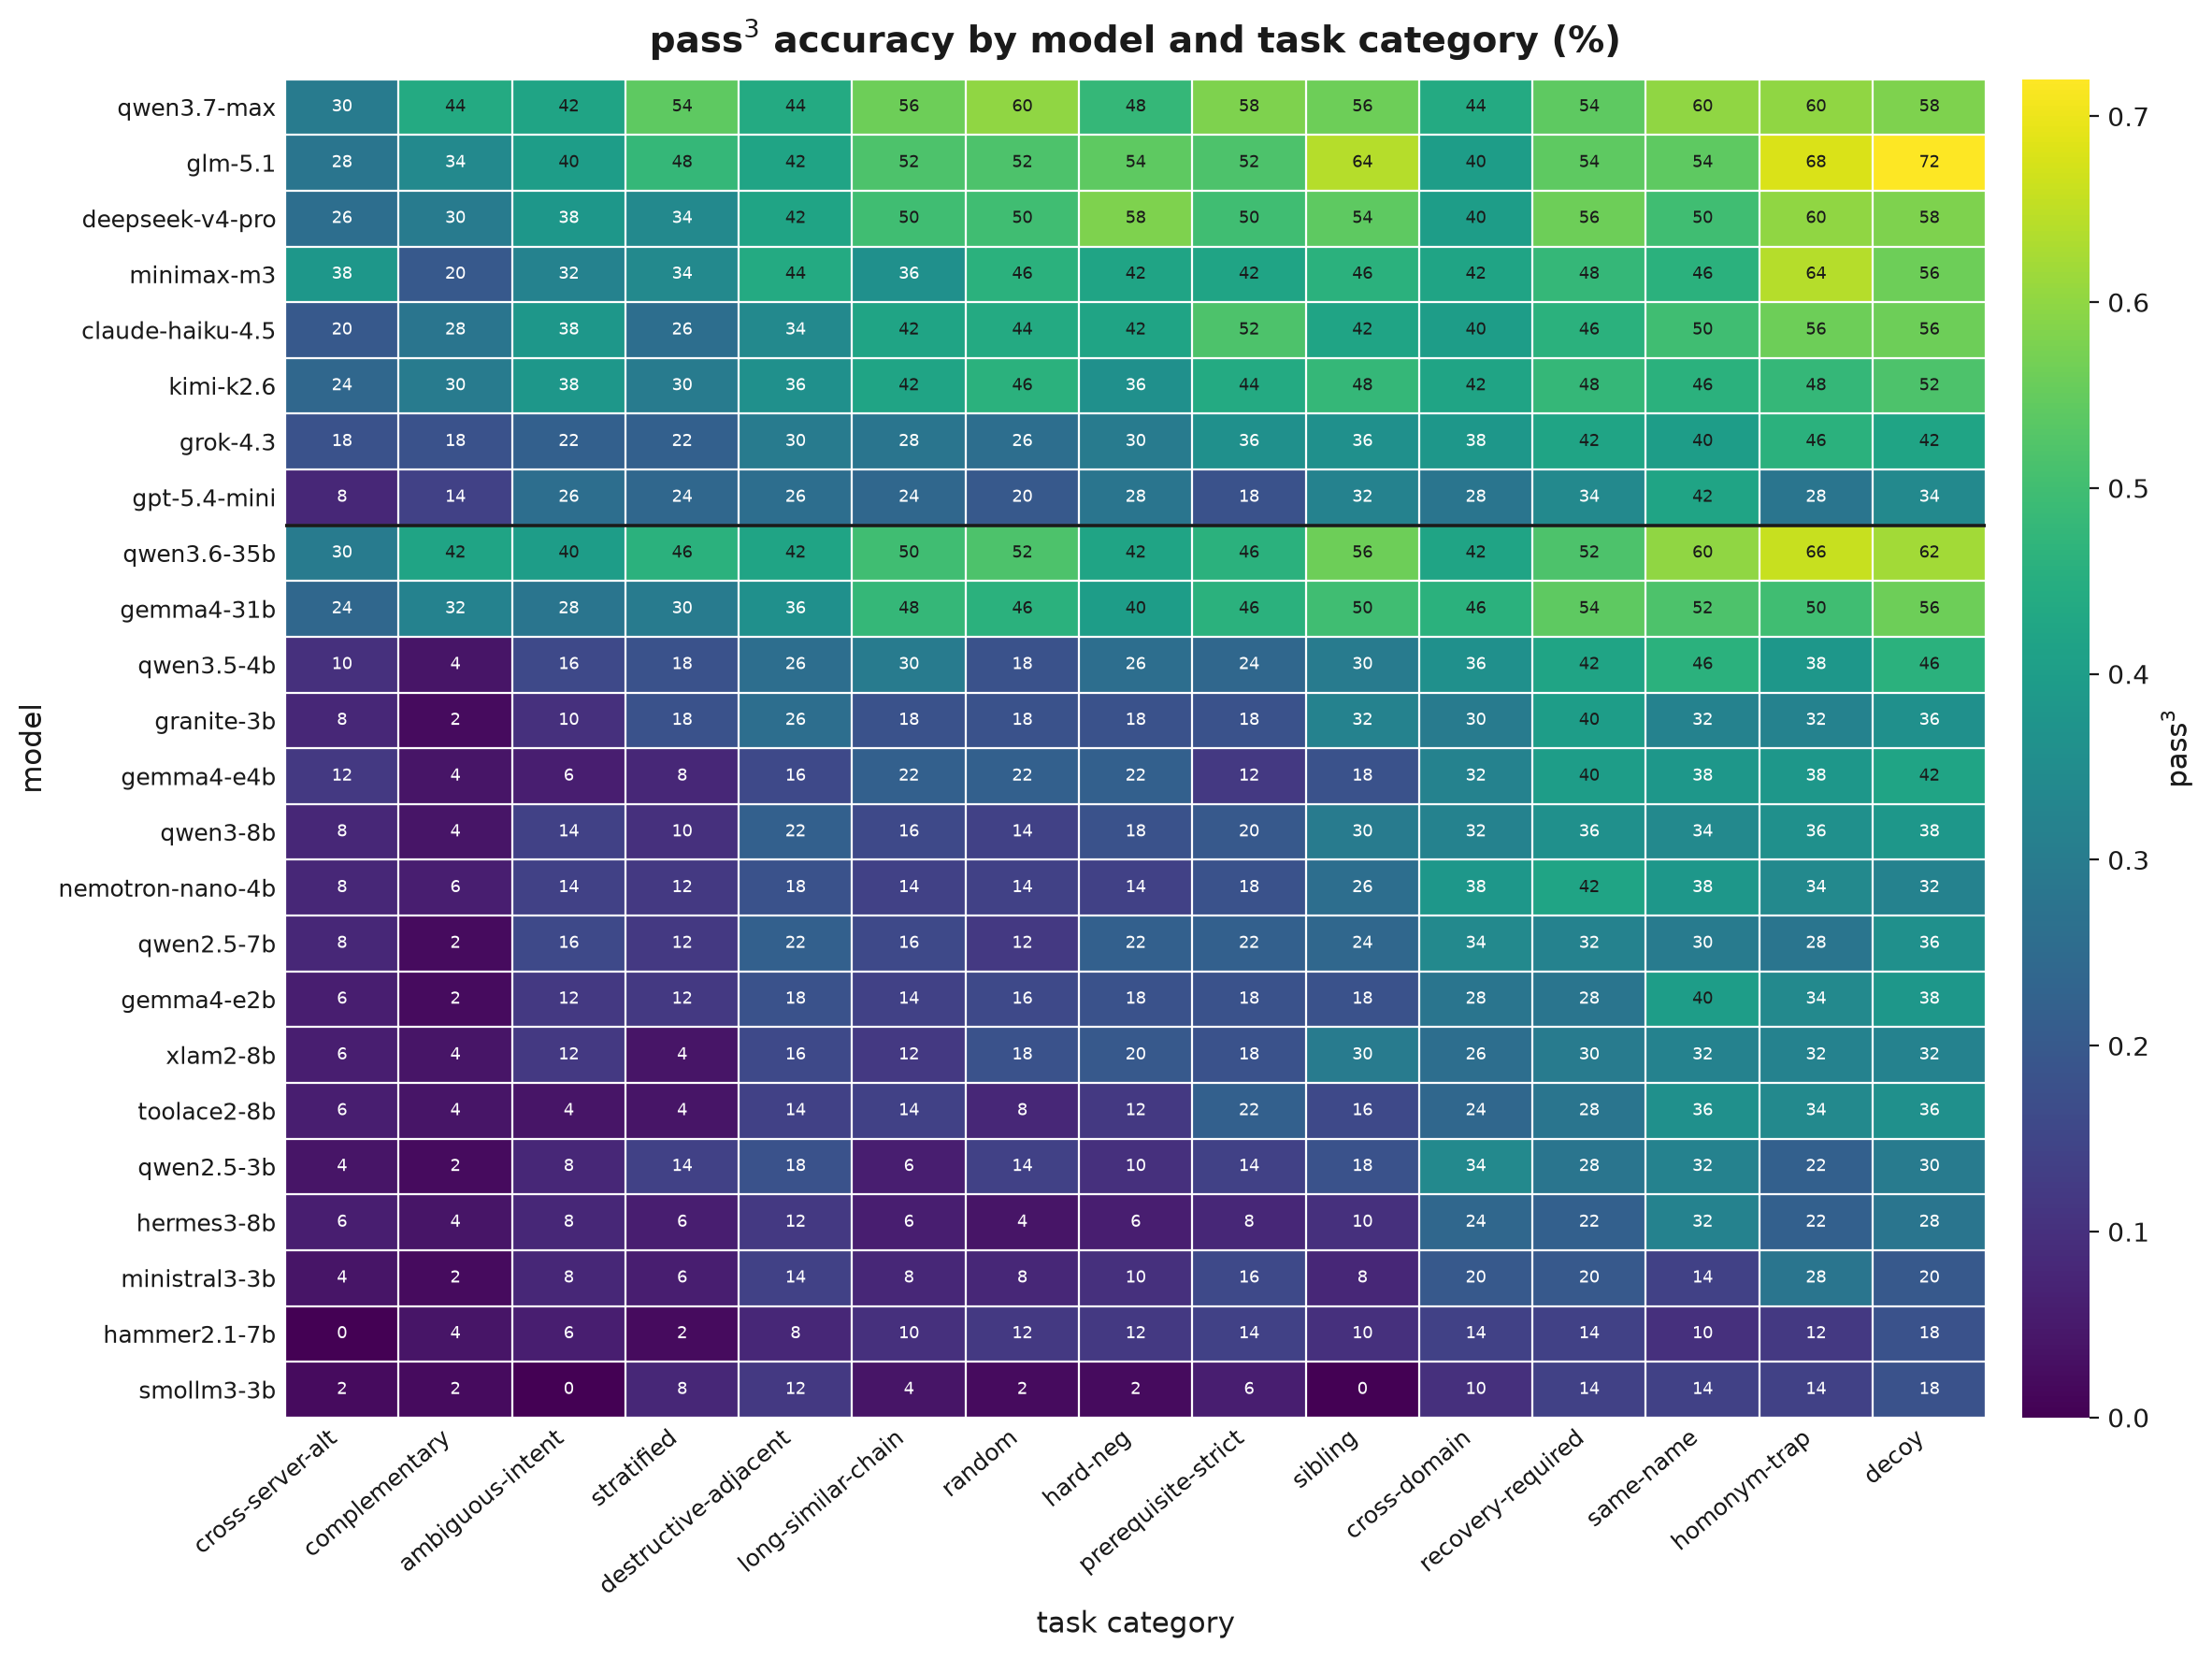
\includegraphics[width=0.97\colwidth]{figures/fig_heatmap.png}
    \end{figure}
    \vspace{-0.4em}
    {\small pass\textasciicircum{}3 by model and category (24 models, 121
    servers, 750 tasks). Difficulty is \emph{vertical} --- some categories are
    hard for every model. \textbf{31\%} of tasks are solved by \emph{no} model,
    only \textbf{2\%} by all.}
  \end{block}

  \begin{block}{Harder as chains get longer}
    \begin{figure}
      \centering
      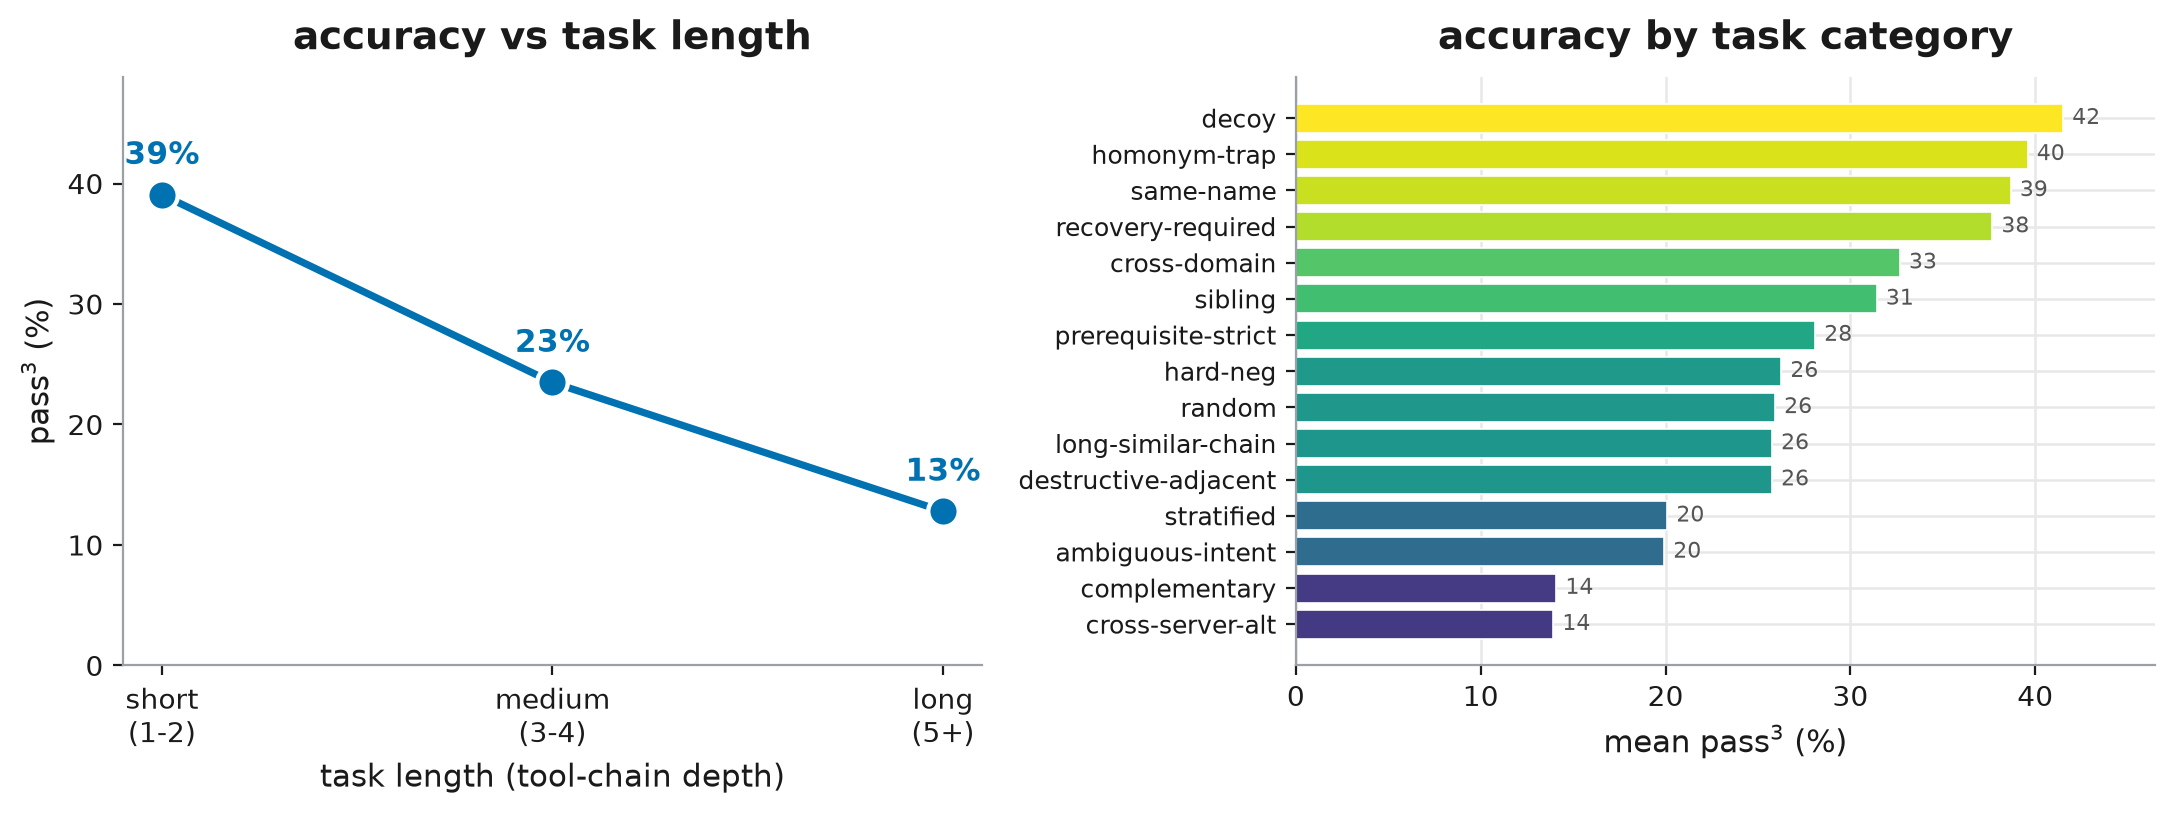
\includegraphics[width=0.78\colwidth]{figures/fig_difficulty.png}
    \end{figure}
    \vspace{-0.4em}
    {\small Accuracy falls with tool-chain length: \textbf{39\%} (1--2 tools)
    $\to$ \textbf{23\%} (3--4) $\to$ \textbf{13\%} (5+). Agents fail by
    \emph{not finishing} long, cross-server jobs --- not by picking the wrong
    tool.}
  \end{block}

  \begin{block}{How agents fail}
    \begin{figure}
      \centering
      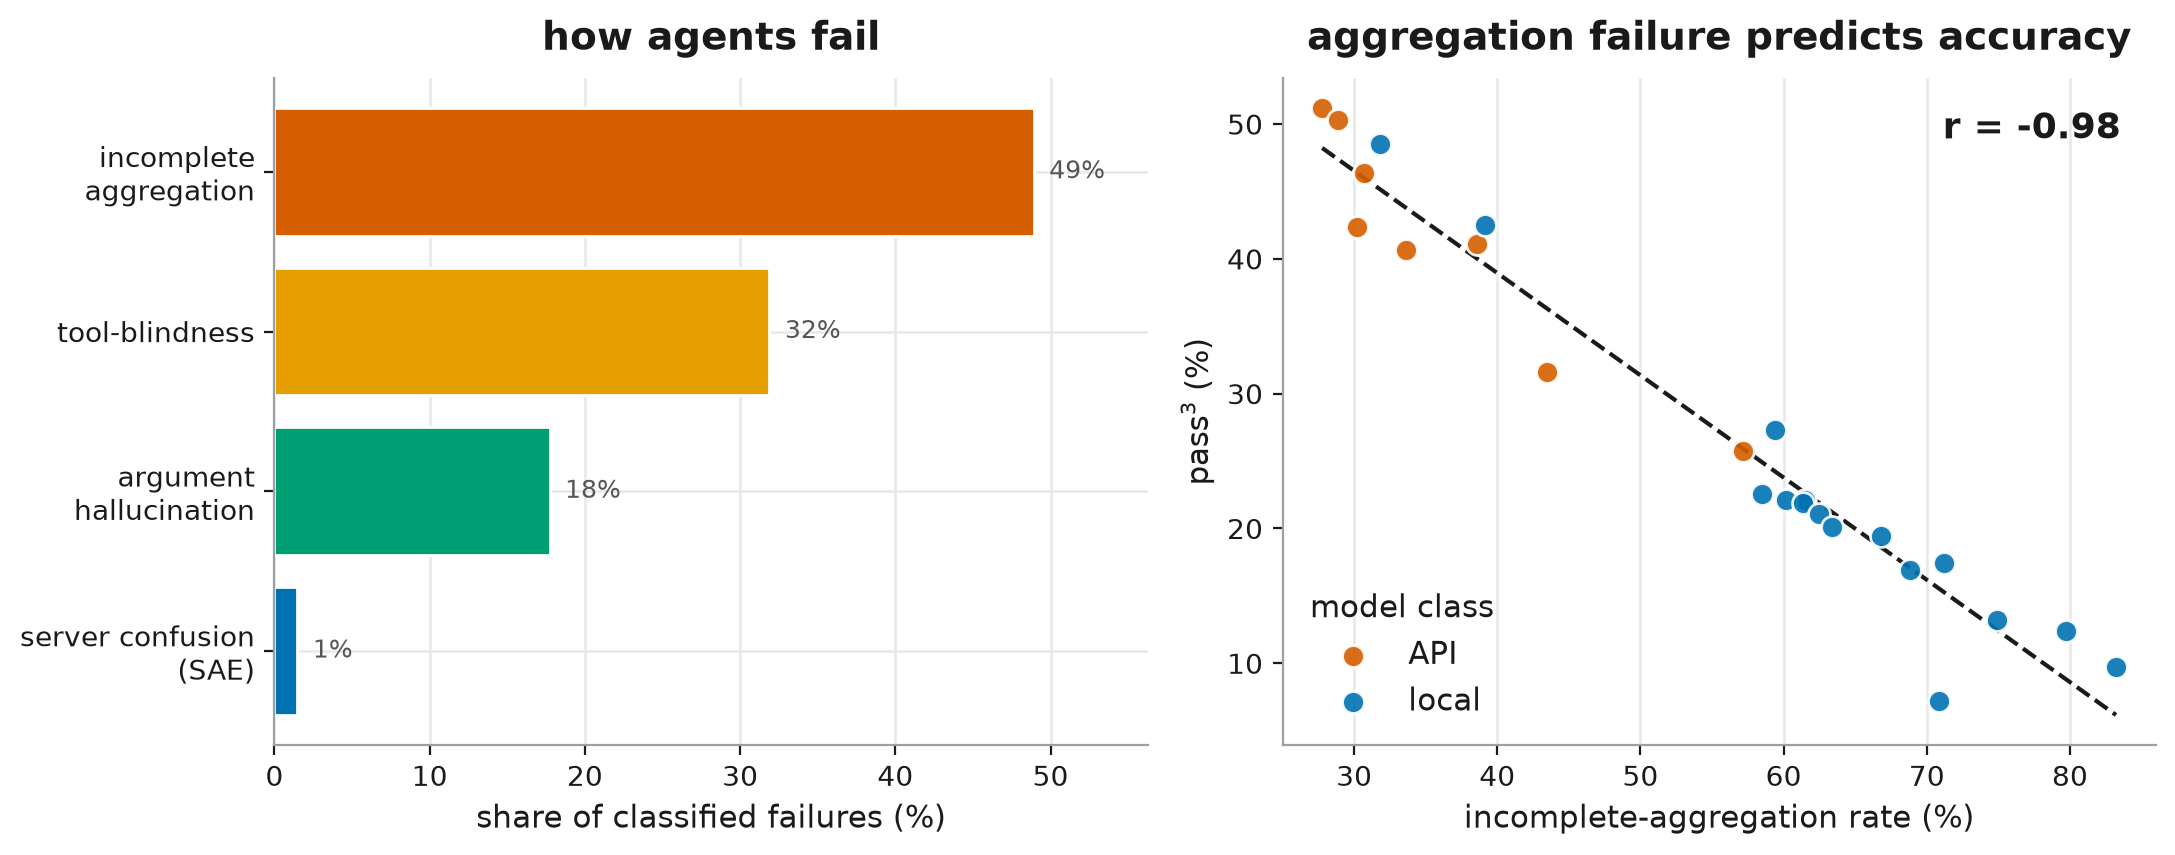
\includegraphics[width=0.82\colwidth]{figures/fig_failure.png}
    \end{figure}
    \vspace{-0.4em}
    {\small Over 54k runs, failures are dominated by \textbf{incomplete
    aggregation} (unmet value checkpoints) and \textbf{tool-blindness}; server
    confusion is near-floor. Incomplete aggregation alone predicts
    pass\textasciicircum{}3 at $r=-0.98$.}
  \end{block}

  \begin{exampleblock}{Paper $\cdot$ Code $\cdot$ Data}
    \begin{columns}[c]
      \begin{column}{0.44\colwidth}
        \centering
        \qrcode[height=8cm]{https://github.com/ITMO-NSS-team/DynamicMCPBench}
      \end{column}
      \begin{column}{0.5\colwidth}
        Scan for the paper, the open-source framework, and the released dataset.
        \\[0.6em]
        Run the benchmark on \emph{your own} MCP servers.
      \end{column}
    \end{columns}
  \end{exampleblock}

\end{column}

\separatorcolumn
\end{columns}
\end{frame}

\end{document}
